
%%%%%%%%%%%%%%%%%%%%%%%%%%%%%%%%%%%%%%%%%%%%%%%%%%%%%%%%%%%%%%%%%%%%%%%%%%%%%%
% This is a template for constructing your project plan document, but
% also to show the use of the l3deliverable class. Use pdflatex and
% bibtex to process the file, creating a PDF file as output (there is
% no need to use dvips when using pdflatex).
%
% Several meta data commands have been implemented to collect
% information such as deliverable identifier, project name etc (see
% below the \date command.

\documentclass{l3deliverable}

%%%%%%%%%%%%%%%%%%%%%%%%%%%%%%%%%%%%%%%%%%%%%%%%%%%%%%%%%%%%%%%%%%%%%%%%%%%%%%
% You can use the svn-multi package to automatically insert version
% control information into your document (an example of how to do this
% is shown below).  Make sure to set the 'svn:keywords' subversion
% property to 'Id' for the source file, for example, type:
%
% svn propset svn:keywords 'Id' d1.tex
%
% in the same directory as your 'd2.tex' file. 
%
% The information between the two $$ will now be updated when you next
% commit the file to your SVN repository.
%
% You can of course, just use this field to insert manual version
% information, e.g. 1.2, 1.2.1 ... instead.


\usepackage{color}
\usepackage{comment}
\usepackage[usenames,dvipsnames,svgnames,table]{xcolor}

%%%%%%%%%%%%%%%%%%%%%%%%%%%%%%%%%%%%%%%%%%%%%%%%%%%%%%%%%%%%%%%%%%%%%%%%%%%%%%

\usepackage{url}

%%%%%%%%%%%%%%%%%%%%%%%%%%%%%%%%%%%%%%%%%%%%%%%%%%%%%%%%%%%%%%%%%%%%%%%%%%%%%%
%% Check these macro values for appropriateness for your own document.

\title{System Design Document}

%%authors
\author{
  Dan Tomosoiu \\
  Peeranat Fupongsiripan \\
  Hector Grebbell \\
  Michael Kilian \\
  Tony Lau \\
}

%%release date 
\date{28 Feb 2013}
\version{2}

\deliverableID{D8.1}
\project{PSD3 Group Exercise 2}
\team{L}

%%%%%%%%%%%%%%%%%%%%%%%%%%%%%%%%%%%%%%%%%%%%%%%%%%%%%%%%%%%%%%%%%%%%%%%%%%%%%%

\begin{document}

%%%%%%%%%%%%%%%%%%%%%%%%%%%%%%%%%%%%%%%%%%%%%%%%%%%%%%%%%%%%%%%%%%%%%%%%%%%%%%

\maketitle

%%%%%%%%%%%%%%%%%%%%%%%%%%%%%%%%%%%%%%%%%%%%%%%%%%%%%%%%%%%%%%%%%%%%%%%%%%%%%%
%% Standard section for all documents

\section{Introduction}

\subsection{Identification}
This document outlines the proposed design for the Internship Management System. 
\subsection{Related Documentation}
\begin{itemize}
\item{Requirements Specification Document (\url{http://fims.moodle.gla.ac.uk/file.php/128/coursework/requirements-specification-ge2.pdf})}
\end{itemize}
 

\subsection{Document Status and Schedule}
30/01/2013 - First Draft\\
27/02/2013 - Final Version
%%%%%%%%%%%%%%%%%%%%%%%%%%%%%%%%%%%%%%%%%%%%%%%%%%%%%%%%%%%%%%%%%%%%%%%%%%%%%%
\section{System Overview}
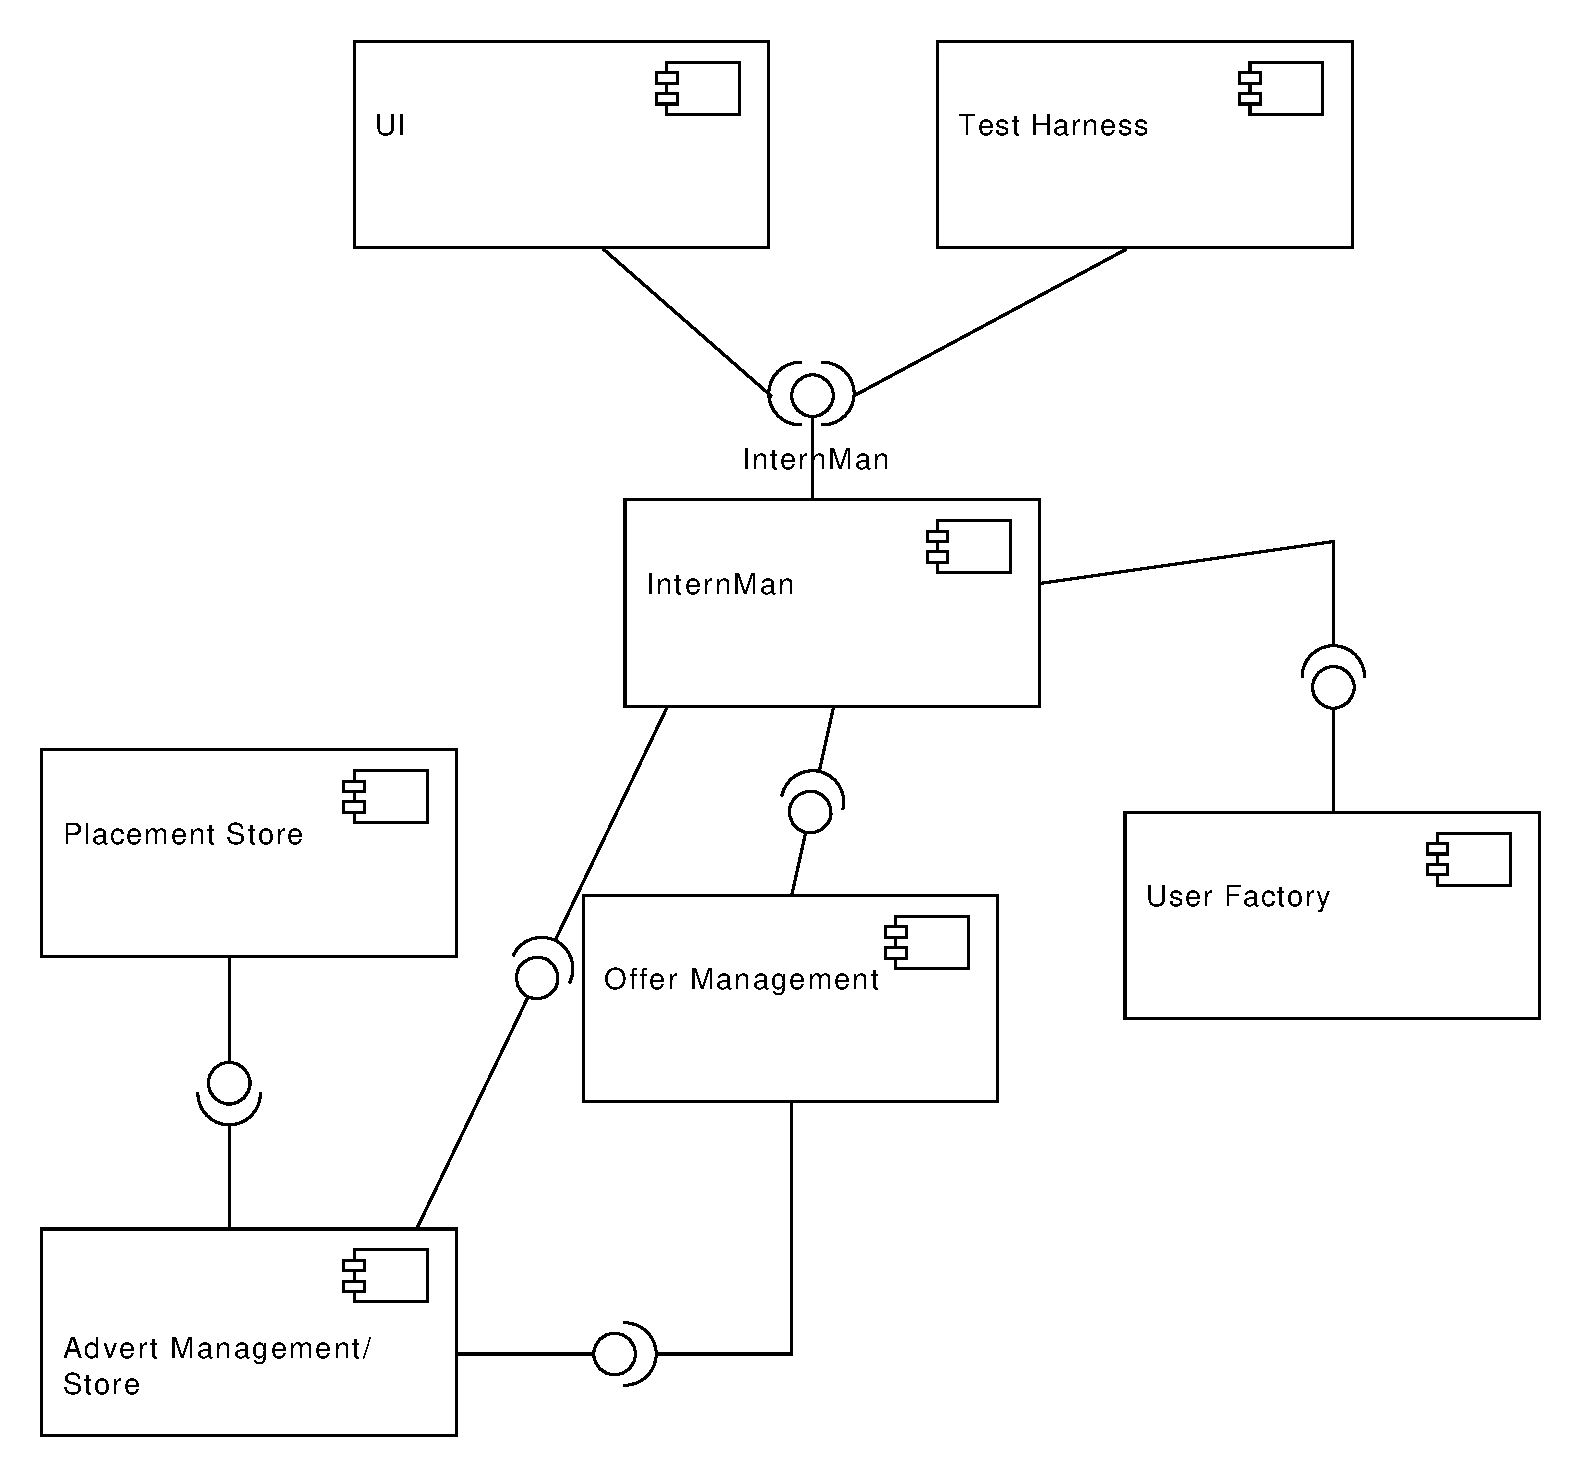
\includegraphics[scale = 0.4]{ComponentDiagram.pdf}\\
The proposed system consists of the following components:
\begin{itemize}
\item{InternMan: This component contains an implementation of the InternMan facade provided and can be seen as the `main' component for the system. }
\item{User Factory: Provides methods for creating new users of different types, storing created users and fetching users from this store. This component also providesservices for authenticating a user's login credentials using a stored username/password combination. Note that this contains the provided UserStore component (not shown).}
\item{Offer Management: Handles offers made to students.}
\item{Advert Management/Store: This component provides the necessary services to create and view adverts, associated these with an employer account, etc. It simultaneously
manages the storage and retrieval of adverts from an appropriate source.}
\item{Placement Store: Provides services for manipulating internships and associating these with an appropriate role.}
\end{itemize}



%%%%%%%%%%%%%%%%%%%%%%%%%%%%%%%%%%%%%%%%%%%%%
\section{State Machine Diagram}
\subsection{Description and Rationale}
The state machine diagram shows the state of objects within the Internship Management System.\\

\subsection{Advertisement State}
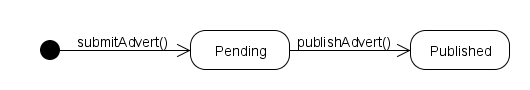
\includegraphics[scale = 0.5]{AdvertState.png}\\

\subsubsection{Rationale}
When an advertisement is created and submitted by the employer it has a pending state.
Only when the course coordinator executes the publishAdvert method does the state of the 
advertisement change from pending to published. The advertisement can be revised prior to
publishing by the course coordinator. \\

\subsection{Student State}
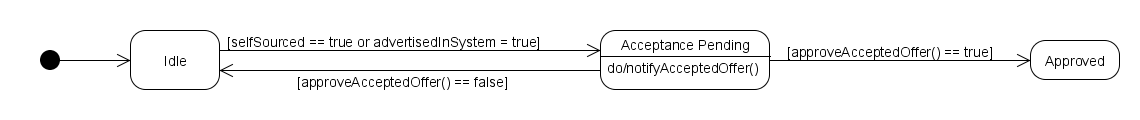
\includegraphics[scale = 0.45]{StudentState.png}\\

\subsubsection{Rationale}
This represents the various states of the student and whether they have an offer which is approved by the course coordinator.
A student will start off in the Idle state and move between this state and the acceptance pending state when they apply for a position advertised in the system
or find a self-sourced role. The final state is Approved which is reached when the course coordinator approves the student's offer which meets the requirements for an
SESP internship. \\  

%%%%%%%%%%%%%%%%%%%%%%%%%%%%%%%%%%%%%%%%%%%%%
%%%%%%%%%%%%%%%%%%%%%%%%%%%%%%%%%%%%%%%%%%%%%
\section{Component Breakdown}

%%%%User factory
\subsection{User Factory}
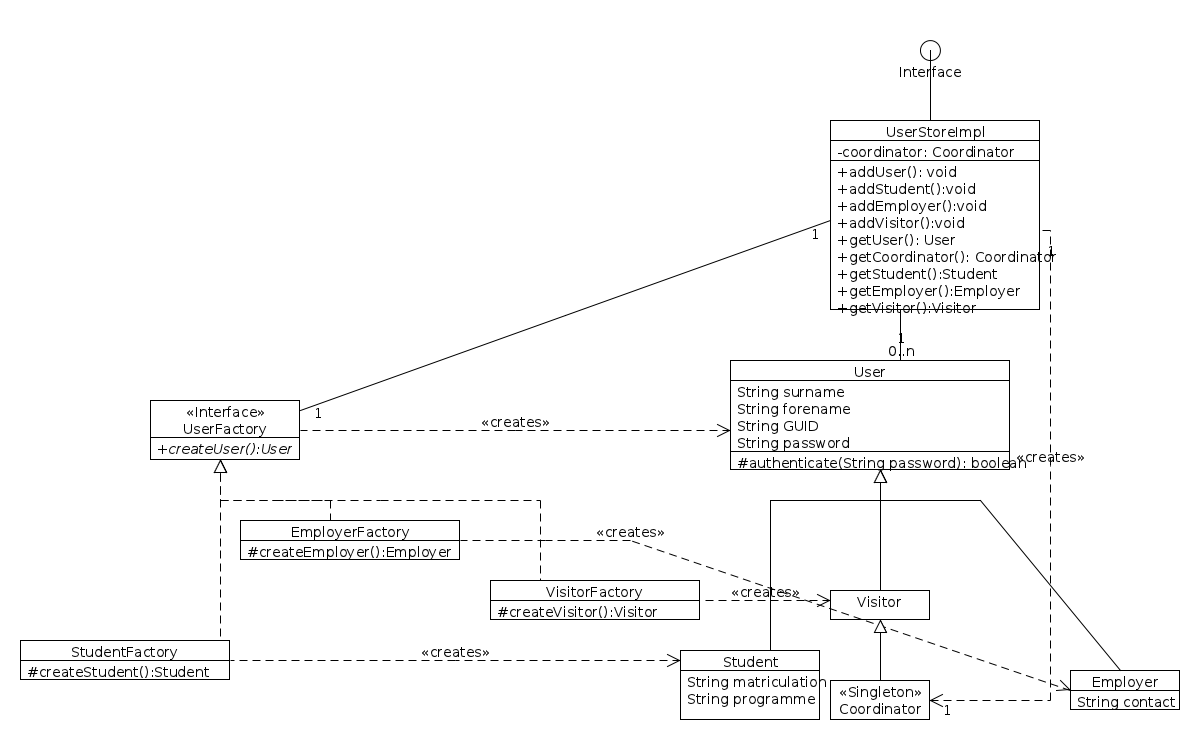
\includegraphics[scale = 0.35]{UserFactoryComponent.png}
\subsubsection{Description and Rationale}
There is a need to create many different categories of user in the system who share attributes and methods. For example all users must be able to log in using a method
to authenticate an input password. In this situation it is appropriate to employ the factory design pattern for the creation of generic users, visitors, students and employers.
The coordinator is not instantiated by a factory, but instead is implemented according to the singleton design pattern. \\
UserStoreImpl groups the methods of these factories and entities together to provide methods for creating and fetching each class of user. For the moment the exact 
means by which these users will be stored has not been decided, but this should also be handled by UserStoreImpl. The method set for UserStoreImpl is equivalent to the API for 
the UserFactory component.
\subsubsection{API}
UserStoreImpl implements UserStore

\textbf{Methods}\\
%addUser
\textbf{public void addUser(String surname, String forename, String GUID, String password)}\\
Adds a new user to the store.\\
\textbf{Parameters}\\
String surname\\
String forename\\
String GUID\\
String password\\
\\
%addVisitor
\textbf{public void addVisitor(String surname,String forename,String GUID, String password)}\\
Adds a new visitor to the store\\
\textbf{Parameters}\\
String surname\\
String forename\\
String GUID\\
String password\\
\\
%addStudent
\textbf{public void addStudent(String surname,String forename,String GUID, String password,String matriculation,String programme)}\\
Adds a new student to the store\\
\textbf{Parameters}\\
String surname\\
String forename\\
String GUID\\
String password\\
String matriculation\\
String programme\\
\\
%addEmployer
\textbf{public void addEmployer(String name, String contact, String password)}\\
Adds a new employer to the store\\
\textbf{Parameters}\\
String name\\
String contact\\
String password\\
\\
%addCoordinator
\textbf{public boolean addCoordinator(String surname, String forename, String GUID, String password)}\\
If one does not exist, a new coordinator is added and true is returned. Else false is returned.
\textbf{Parameters}\\
String surname\\
String forename\\
String GUID\\
String password\\
\\
%getUser
\textbf{public User getUser(String GUID, String password)}\\
Returns a user specified by the GUID, if authentication is successful.\\
\textbf{Return} the user specified by GUID, if the password is a match\\
\textbf{Parameters}\\
String GUID\\
String password\\
\\
%getVisitor
\textbf{public Visitor getVisitor(String GUID, String password)}\\
Returns a visitor specified by the GUID, if authentication is successful.\\
\textbf{Return} the visitor specified by GUID, if the password is a match\\
\textbf{Parameters}\\
String GUID\\
String password\\
\\
%getStudent
\textbf{public Student getStudent(String GUID, String password)}\\
Returns a Student specified by the GUID, if authentication is successful.\\
\textbf{Return} the student specified by GUID, if the password is a match\\
\textbf{Parameters}\\
String GUID\\
String password\\
\\
%getEmployer
\textbf{public Visitor getEmployer(String contact, String password)}\\
Returns an employer specified by the contact if authentication is successful.\\
\textbf{Return} the employer specified by contact, if the password is a match\\
\textbf{Parameters}\\
String contact\\
String password\\
\\
%getCoordinator
\textbf{public Visitor getCoordinator()}\\
Returns the coordinator instance.\\
\textbf{Return} the coordinator instance\\
\textbf{Parameters}\\
String contact\\
String password\\
\\

%getUserMap
\textbf{public Map\textless String,User\textgreater  getUserMap()}\\
Returns map holding all current users.\\
\textbf{Return} The user store's user map.\\
\textbf{Parameters}\\
N/A
\\


%getVisitorMap
\textbf{public Map\textless String,Visitor\textgreater   getVisitorMap()}\\
Returns map holding all current visitors.\\
\textbf{Return} The user store's visitor map.\\
\textbf{Parameters}\\
N/A
\\

%getStudentMap
\textbf{public Map\textless String,Student\textgreater   getStudentMap()}\\
Returns map holding all current students.\\
\textbf{Return} The user store's student map.\\
\textbf{Parameters}\\
N/A
\\

%getEmployerMap
\textbf{public Map\textless String,Employer\textgreater   getUserMap()}\\
Returns map holding all current employer.\\
\textbf{Return} The user store's employer map.\\
\textbf{Parameters}\\
N/A
\\
%%%%%OfferManager
\subsection{Offer Management}
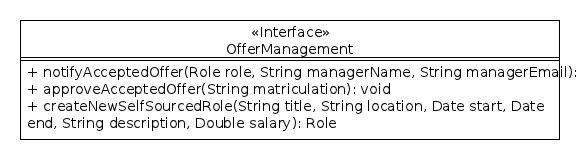
\includegraphics[scale = 0.5]{OfferManagement.png}
\subsubsection{Description and Rationale}
This component is needed to allow students to notify the course coordinator that they have accepted an internship. If the internship was advertised in the internship management system, then it is automatically approved. Otherwise, the student can create a new self-sourced role which will send an email to the course coordinator asking for approval. Approval is done through this component.
\subsubsection{API}
OfferMangementImpl implements OfferManagement\\
\textbf{Methods}\\

\textbf{public void notifyAcceptedOffer(Role role, String managerName, String managerEmail)}\\
Sends email to coordinator informing that a student has accepted an internship\\
\textbf{Parameters}\\
Role role\\
String managerName\\
String managerEmail\\
\\

\textbf{public void approveAcceptedOffer(String matriculation)}\\
Sends email to coordinator informing that a student has accepted an internship\\
\textbf{Parameters}\\
String matriculation\\
\\
\textbf{public Role createNewSelfSourcedRole(String title, String location, Data start, Date end, String description, Double salary)}\\
Sends email to coordinator informing that a student has accepted an internship\\
\textbf{Return}\\
Returns the newly created self-sourced role\\
\textbf{Parameters}\\
String title\\
String location\\
Data start\\
Date end\\
String description\\
Double salary\\
\\

%%%%%Advert Management/Store
\subsection{Advert Management/Store}
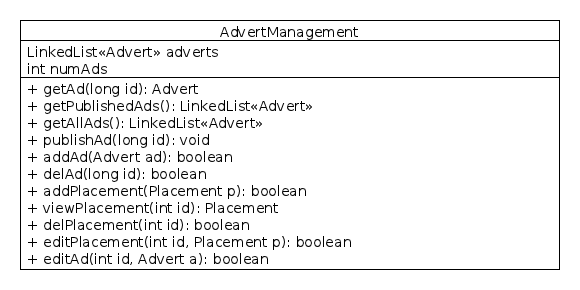
\includegraphics[scale = 0.5]{adStore.png}

\subsubsection{Description and Rationale}
Advert Management/Store is needed to handle creation, selection and publishing of all advertisements within the system. It interacts with other components which need information on adverts through the selectAdvertisement method which provides a handle on an advert with a supplied index.
\subsubsection{API}
\textbf{public Advertisement getAd (long id)}\\
Retrives advert indexed by id.\\
\textbf{Return}\\
Advertisement advert\\
\textbf{Parameters}\\
long id\\
\\

\textbf{public LinkedList\textless Advertisement\textgreater   getPublishedAds()}\\
Retrives list of all published adverts\\
\textbf{Return}\\
LinkedList\textless Advertisement\textgreater   adverts.\\
\textbf{Parameters}\\
N/A\\
\\

\textbf{public LinkedList\textless Advertisement\textgreater   getAllAds()}\\
Retrives list of all adverts\\
\textbf{Return}\\
LinkedList\textless Advertisement\textgreater   adverts.\\
\textbf{Parameters}\\
N/A\\
\\

\textbf{public void publishAd (long id)}\\
Publishes advert indexed by id.\\
\textbf{Return}\\
void\\
\textbf{Parameters}\\
long id\\
\\

\textbf{public boolean addAd (Advertisement ad)}\\
Adds new advert to store\\
\textbf{Return}\\
true if added successfully, false otherwise.\\
\textbf{Parameters}\\
Advertisement ad\\
\\

\textbf{public boolean delAd (long id)}\\
Deletes advert indexed by id.\\
\textbf{Return}\\
True if advert found and deleted, false otherwise.\\
\textbf{Parameters}\\
long id\\
\\

\textbf{public boolean editAd (int id,Advert a)}\\
Edit advert indexed by id to match a \\
\textbf{Return}\\
true if found and edited successfully, false otherwise.\\
\textbf{Parameters}\\
int id\\
Placement p\\
\\


\textbf{public boolean addPlacement (Placement p)}\\
Adds new placement to the store.\\
\textbf{Return}\\
true if added successfully, false otherwise.\\
\textbf{Parameters}\\
Placement p\\
\\

\textbf{public Placement viewPlacement (int id)}\\
Return placement identified by id\\
\textbf{Return}\\
Placement indexed by id if it exists, null otherwise.\\
\textbf{Parameters}\\
int id\\
\\

\textbf{public boolean editPlacement (int id,Placement p)}\\
Edit placement identified by id to match p\\
\textbf{Return}\\
true if found and edited, false otherwise\\
\textbf{Parameters}\\
int id\\
Placement p\\
\\


%%%%%Placement Store
\subsection{Placement Store}
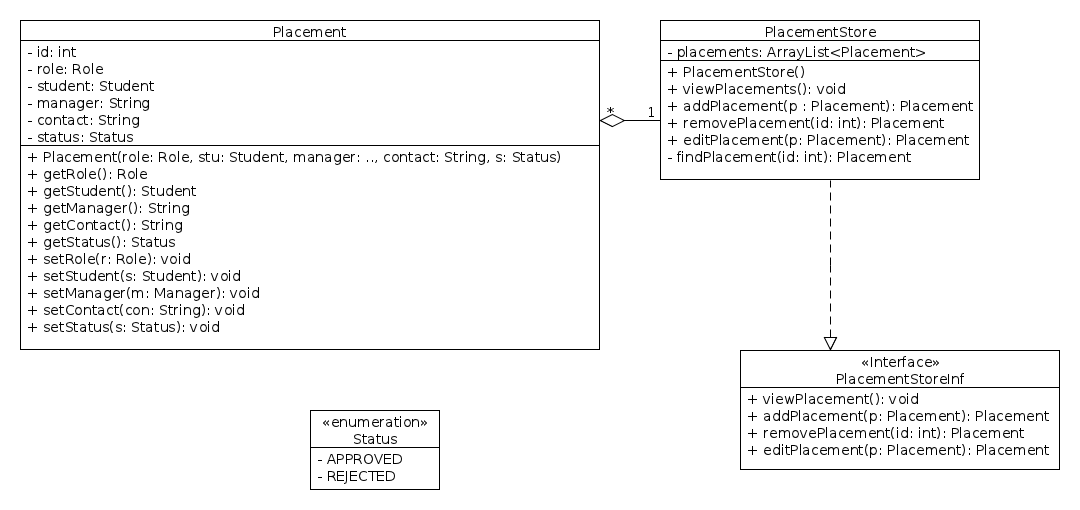
\includegraphics[scale = 0.4]{ClassDiagram_PlacementStore.png}
\subsubsection{Description and Rationale}
Placement Store contains all information on placements in the system at any given time and is needed to allow other components to keep track of which placements are in the system and their status.
\subsubsection{API}
\textbf{Interface PlacementStoreInf}\\

\textbf{Methods}\\
%viewPlacements
\textbf{public void viewPlacements()}\\
Prints out all existing placements.\\
\\
%addPlacement
\textbf{public Placement addPlacement( Placement p )}\\
Add new placement.\\
\textbf{Return: }Placement p added if successful, otherwise null.\\
\textbf{Parameters}\\
Placement p\\
\\
%removePlacement
\textbf{public Placement removePlacement(int id)}\\
\textbf{Return: }Placement with identification number id removed if successful , otherwise null.\\
\textbf{Parameters}\\
int id\\
\\
%editPlacement
\textbf{public Placement editPlacement(Placement p) }\\
Edits existing placement.\\
\textbf{Return: }Placement edited if successful, null otherwise.\\
\textbf{Parameters}\\
Placement p\\
\\
%%%%Class Placement
\textbf{Class Placement}\\
Contains details about the internship including the student taking and role involved.\\
\\
\textbf{public Placement(Role role, Student student, String manager , String contact, Status status)}\\
\textbf{Parameters}\\
Role role\\
Student student\\
String manager\\
String contact\\
Status status\\
\\
\textbf{public Role getRole()}\\
\textbf{Return: }Role of placement if exists, null otherwise.\\
\\
\textbf{public Student getStudent()}\\
\textbf{Return: }Student secured the placement , null otherwise.\\
\\
\textbf{public String getManager()}\\
\textbf{Return:}Manager if exists, null otherwise.\\
\\
\textbf{public String getContact()}\\
\textbf{Return: }Contact details, if exists, null otherwise.\\
\\
\textbf{public Status getStatus()}\\
\textbf{Return: }returns the status of a particular placement (value can be either APPROVED OR REJECTED)\\
\\
\textbf{setRole(Role r)}\\
\textbf{Return:}\\
\textbf{Parameters}\\
Role r\\
\\
\textbf{setStudent(Student s)}\\
\textbf{Return:}\\
\textbf{Parameters}\\
Student s\\
\\
\textbf{setManager(String m)}\\
\textbf{Return:}\\
\textbf{Parameters}\\
String m
\\
\textbf{setContact(String c)}\\
\textbf{Return:}
\textbf{Parameters}
String c\\
\\
\textbf{setStatus(Status s)}\\
\textbf{Return:}\\
\textbf{Parameters}\\
Status s\\
\\
%%%%%%%%%%%%%%%%%%%%%%%%%%%%%%%%%%%%%%%%%%%%%%%%%%%%%%%%%%%%%%%%%%%%%%%%%%%%%%

\appendix

%Including expansions of non-standard abbreviations and acronyms and
%other key definitions.  You may find it useful to maintain a glossary
%as a shared section amongst all your PSD documents. using the
%%API  - Application programming interface\\
PSD  - Professional Software Development\\
PSD3 - Professional Software Development 3\\
UML  - Unified Modeling Language\\

\section{Glossary}
\begin{itemize}
\item{UML - Unified Modelling Language}
\item{API - Application Programming Interface}
\item{PSD/PSD3 - Professional Software Development (3)}
\end{itemize}

\end{document}
%%%%%%%%%%%%%%%%%%%%%%%%%%%%%%%%%%%%%%%%%%%%%%%%%%%%%%%%%%%%%%%%%%%%%%%%%%%%%%
